\documentclass[conference]{IEEEtran}
\IEEEoverridecommandlockouts
% The preceding line is only needed to identify funding in the first footnote. If that is unneeded, please comment it out.
\usepackage{cite}
\usepackage{amsmath,amssymb,amsfonts}
\usepackage{algorithmic}
\usepackage{graphicx}
\usepackage{textcomp}
\usepackage{xcolor}
\usepackage{float}
\usepackage{tikz}
\usepackage{pgfplots}
\pgfplotsset{compat=1.17}


\def\BibTeX{{\rm B\kern-.05em{\sc i\kern-.025em b}\kern-.08em
    T\kern-.1667em\lower.7ex\hbox{E}\kern-.125emX}}
\begin{document}

\title{WoahACPU: CPU Scheduler Simulator}

\author{
  \IEEEauthorblockN{Othmane AZOUBI}
  \IEEEauthorblockA{
    College of Computing\\
    Mohammed VI Polytechnic University\\
    Benguerir, Morocco\\
  }
  \and
  \IEEEauthorblockN{Mohammed-Rida ELHANI}
  \IEEEauthorblockA{
    College of Computing\\
    Mohammed VI Polytechnic University\\
    Benguerir, Morocco\\
  }
}


\maketitle

\begin{abstract}
This report is a brief summary of the project, written with love \& care. We aimed to keep it concise and focused on core ideas and clarity rather than excessive length.

The project simulates five CPU‑scheduling algorithms—FCFS, SJF, Priority, Round Robin, and Priority + RR—using the Unity engine. Workloads are defined by arrival time, burst time, and priority. Input can come from a JSON file or be randomly generated. The system measures metrics such as waiting time and turnaround time so you can compare each algorithm’s trade‑offs in throughput, fairness, and responsiveness.
\end{abstract}

\section{Project Architecture}

\subsection{Overall Architecture}

Figure~\ref{fig:architecture} shows that the system is divided into two main components:
\begin{itemize}
  \item \textbf{Unity Client:} The core simulator and user‐interface. It animates processes on the CPU, lets the user start, pause, or adjust the simulation speed, and displays which processes are executing.
  \item \textbf{Flask Backend:} Responsible for generating processes (either randomly or from a file), collecting benchmarking metrics. Process are exposed via RESTful endpoints to the Unity client.
\end{itemize}

\begin{figure}[H]
    \centering
    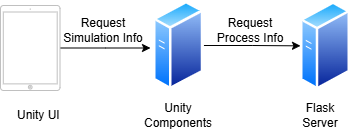
\includegraphics[width=0.8\linewidth]{apah.png}
    \caption{System Architecture}
    \label{fig:architecture}
\end{figure}


\subsection{Motivation for Design Choices}
Basically, we had two ideas. The first was to implement the scheduler in an object‑oriented language so we could leverage design patterns and apply what we’ve learned in our software‑development course. The second was to create an interactive visualization—so you can actually see which process is occupying the CPU and watch the “hardware” timer discussed in Section II.C

We considered many languages: Python, LUA, C++, Java, and Csharp. We ruled out Python because it would make the project too easy and we wouldn’t learn the problem‑solving skills this project requires. We didn’t want Java, since we’ve already 'had enough' with Spring Boot. Although LUA (via CoronaSDK or LÖVE) would be fast and would support our interactive‑visualization idea, it’s hard to simulate true OOP in Lua (No real OOP—it’s just simulated using tables and metatables). C++ is a strong choice—but I expect most of our classmates will pick it, and we’d like our project to stand out. That leaves Csharp with the Unity engine for visualization.

\subsection{Class Diagram}

\begin{figure}[H]
    \centering
    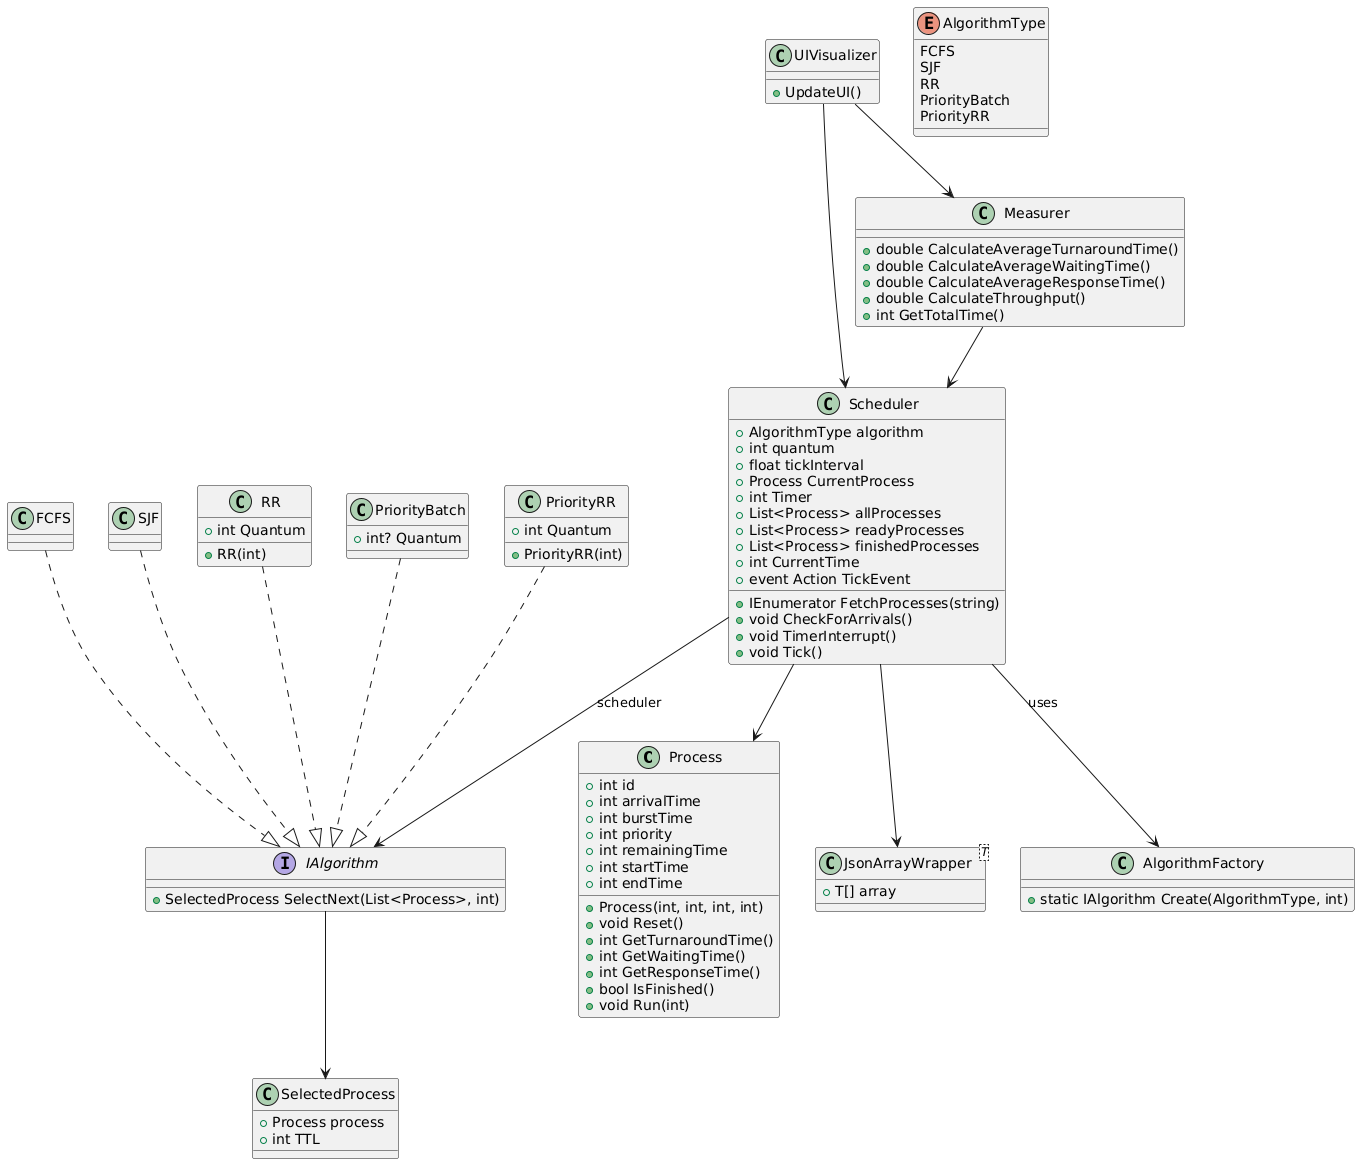
\includegraphics[width=0.9\linewidth]{UML.png}
    \caption{Class Diagram}
    \label{fig:UML}
\end{figure}

\subsection{End Points}
\begin{itemize}
  \item \textbf{GET /}  
    \begin{itemize}
      \item Reads \texttt{processes.json} and returns its contents.  
      \item \textbf{Responses:}
      \begin{itemize}
        \item 200 OK: JSON array of process objects  
        \item 500 Internal Server Error: if the file cannot be read or parsed  
      \end{itemize}
    \end{itemize}

  \item \textbf{POST /generate}  
    \begin{itemize}
      \item Creates a list of random processes based on the JSON payload.  
      \item \textbf{Example Request JSON:}
      \begin{verbatim}
{
  "minburst": 1,
  "maxburst": 10,
  "minarrival": 0,
  "maxarrival": 20,
  "minpriority": 1,
  "maxpriority": 5,
  "count": 5
}
      \end{verbatim}
      \item \textbf{Responses:}
      \begin{itemize}
        \item 200 OK: JSON array of generated processes, sorted by arrival time  
        \item 400 Bad Request: missing body, wrong types, or min $>$ max  
      \end{itemize}
    \end{itemize}

  \item \textbf{POST /benchmark}  
    \begin{itemize}
      \item Stores performance results for one algorithm in server memory.  
      \item \textbf{Example Request JSON:}
      \begin{verbatim}
{
  "algorithm": "RR",
  "metrics": {
    "avg_wait": 12.3,
    "avg_turnaround": 20.5,
    other metrics etc....
  }
}
      \end{verbatim}
      \item \textbf{Responses:}
      \begin{itemize}
        \item 201 Created: \texttt{\{"status":"ok"\}}  
        \item 400 Bad Request: if “algorithm” or “metrics” is missing  
      \end{itemize}
    \end{itemize}

  \item \textbf{GET /benchmark}  
    \begin{itemize}
      \item Renders an HTML page with a table of all stored results. And displays them as nice graphs and charts for comparaison.
      \item \textbf{Response:}
      \begin{itemize}
        \item 200 OK: HTML page showing algorithms and their metrics  
      \end{itemize}
    \end{itemize}
\end{itemize}


\section{Design Choices}
The system is designed carefully to respect Modularity, Seperation of concerns and SOLID principles here is how it is done:
\subsection{Structs \& Interfaces}
Before we proceed we'd like to defend our structure choices from Section I.C:
\begin{itemize}
  \item It is not needed to repeat the definition of a process entry; the Class Diagram already makes it clear.
  \item \textbf{Enum \texttt{AlgorithmType}}\\
    Lists the possible algorithm types. This avoids using messy string comparisons.
  \item \textbf{Interface \texttt{IAlgorithm}}\\
    Holds any scheduling algorithm as a “strategy.” This lets us use the Strategy pattern and keeps the core scheduler simple. The scheduler only calls the method \texttt{SelectNext} and does not need to know which algorithm runs. This also follows the Single Responsibility Principle: the scheduler moves processes and handles timer interrupts, and each algorithm class only picks the next process.
  \item \textbf{Struct \texttt{SelectedProcess}}\\
    Contains the data that an algorithm returns. At first, we thought about returning only the \texttt{Process}, but then the scheduler would not know how long that process should run before the next interrupt. This is important because the scheduler does not know if the algorithm is preemptive or not.
  \item \textbf{Class \texttt{AlgorithmFactory}}\\
    Uses the Factory pattern to make \texttt{IAlgorithm} objects. This keeps the scheduler from having to change when we add or remove algorithms.
\end{itemize}

\subsection{Flask Server}
We’ll cover the Flask server now, since the next subsection refers back to it. The endpoints are defined in Section I.D, where their functionality is already explained.

We chose this approach to keep Unity from handling file I/O on our systems—it would complicate the production build process. With a Flask server, we can change the I/O handling at any time without rebuilding or updating the Unity code.

A second reason is that, with our experience using Unity, we know that its random‑number generation can become predictable and is tricky to fix. Python’s random‑number libraries are simpler and more reliable for this task.

Finally, this approach will simplify stress testing.

\subsection{Scheduler}
In this subsection, we describe the simulation's main component: the scheduler. The scheduler class is a state machine with three main states summarized in Figure ~\ref{fig:statemachine}

\paragraph{State 1: Begin} 

In this phase, the system fetches processes from the Flask server and caches them. All scheduler attributes are reset to their initial values (empty or zero). The processes remain in cache until State 3 loads them into the process table. Then the scheduler moves to State 2.

\paragraph{State 2: Scheduling Decision}  
Here the scheduler is faced with two decisions:
\begin{itemize}
  \item If the timer expires and the process still has remaining time (remaining time $>$ 0), the scheduler returns it to the ready queue.
  \item Otherwise, it moves the process to the finished queue for later benchmarking.
\end{itemize}
Then scheduler applies the \texttt{IAlgorithm.SelectNext} strategy to choose the next process. It updates its timer and gives CPU control to that process (Moves to State 3)  


\paragraph{State 3: CPU Tick}  

This state simulates the CPU itself. We combine it with the scheduler code to avoid overcomplicating the implementation. The \texttt{void Tick()} function does the following:
\begin{enumerate}
  \item Checks for new arrivals by scanning the cache from State 1. Any process whose arrival time equals the current time is added to the ready queue.
  \item Executes one CPU instruction (one “tick”). The tick frequency is defined by a class attribute.
  \item If the hardware timer expires (timer = 0) or the process finishes executing (remaining time = 0), the simulated hardware issues a \texttt{TimerInterrupt()} event and returns control to the scheduler (Moves to State 2).
  \item After each tick, a \texttt{TickEvent} is invoked to update the UI so users can see what is happening.
\end{enumerate}

\begin{figure}[H]
    \centering
    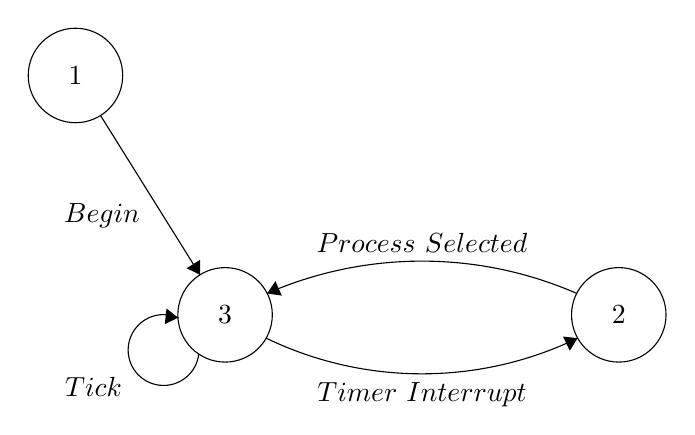
\begin{tikzpicture}[scale=0.2]
        \tikzstyle{every node}+=[inner sep=0pt]
        \draw [black] (23.6,-10.7) circle (3);
        \draw (23.6,-10.7) node {$1$};
        \draw [black] (58.1,-25.9) circle (3);
        \draw (58.1,-25.9) node {$2$};
        \draw [black] (33.1,-25.9) circle (3);
        \draw (33.1,-25.9) node {$3$};
        \draw [black] (25.19,-13.24) -- (31.51,-23.36);
        \fill [black] (31.51,-23.36) -- (31.51,-22.41) -- (30.66,-22.94);
        \draw (27.72,-19.59) node [left] {$Begin$};
        \draw [black] (55.493,-27.38) arc (-64.1961:-115.8039:22.727);
        \fill [black] (55.49,-27.38) -- (54.56,-27.28) -- (54.99,-28.18);
        \draw (45.6,-30.15) node [below] {$Timer\mbox{ }Interrupt$};
        \draw [black] (35.77,-24.537) arc (113.55423:66.44577:24.598);
        \fill [black] (35.77,-24.54) -- (36.7,-24.68) -- (36.3,-23.76);
        \draw (45.6,-21.99) node [above] {$Process\mbox{ }Selected$};
        \draw [black] (31.43,-28.378) arc (-6.25512:-294.25512:2.25);
        \draw (26.58,-30.47) node [left] {$Tick$};
        \fill [black] (30.12,-26.08) -- (29.38,-25.5) -- (29.27,-26.49);
    \end{tikzpicture}
    \caption{Scheduler Class as a State Machine}
    \label{fig:statemachine}
\end{figure}

\subsection{Measurer}
This class is simple: it reads from the finished queue and collects measurements like arrival time, start time, finish time, etc.. And then compute the evaluation metrics that the UI component will display in its text boxes.
\subsection{Algorithms}
I left this part at the end since it just repeats the textbook. The implemented algorithm strategies are as follows:
\begin{itemize}
  \item \textbf{FCFS}\\
    Processes are handled in the order they arrive. No preemption: once a process starts, it runs until completion. Simple but can lead to long waits (convoy effect).
  \item \textbf{SJF}\\
    Picks the process with the smallest total service time next. It is non‑preemptive (runs to completion). Minimizes average wait time but requires knowing job lengths in advance. Also can lead to starving long length jobs.
  \item \textbf{RR (Round‑Robin)}\\
    Each process runs for a fixed time slice (quantum). If it doesn’t finish, it goes to the back of the ready queue. Ensures fairness and good responsiveness for time‑sharing systems.
  \item \textbf{PriorityBatch}\\
    Processes have static priorities; the scheduler picks the highest‑priority job next. Non‑preemptive: once started, a job runs until completion. Can starve low‑priority jobs.
  \item \textbf{PriorityRR}\\
    Combines priority scheduling with time‑slicing. Within each priority level, processes share the CPU in round‑robin fashion. Balances priority treatment with fairness.
\end{itemize}

\section{Testing \& Preview}

\subsection{Test Case}
Simulation Screenshots are demonstrated in Figure~\ref{fig:mid-sim} \& ~\ref{fig:end-sim}

A list of processes used in the simulation (View \texttt{processes.json} (quantum = 2 for RR and Priority+RR):

\begin{table}[H]
  \centering
  \caption{Process Attributes}
  \label{tab:processes}
  \begin{tabular}{ccccc}
    \hline
    ID & Arrival Time & Burst Time & Priority & Remaining Time\\ \hline
     1 & 0            & 8          & 3        & 8             \\
     2 & 2            & 4          & 1        & 4             \\
     3 & 4            & 9          & 2        & 9             \\
     4 & 6            & 5          & 4        & 5             \\
     5 & 8            & 2          & 1        & 2             \\
    \hline
  \end{tabular}
\end{table}

\begin{figure}[H]
  \centering
  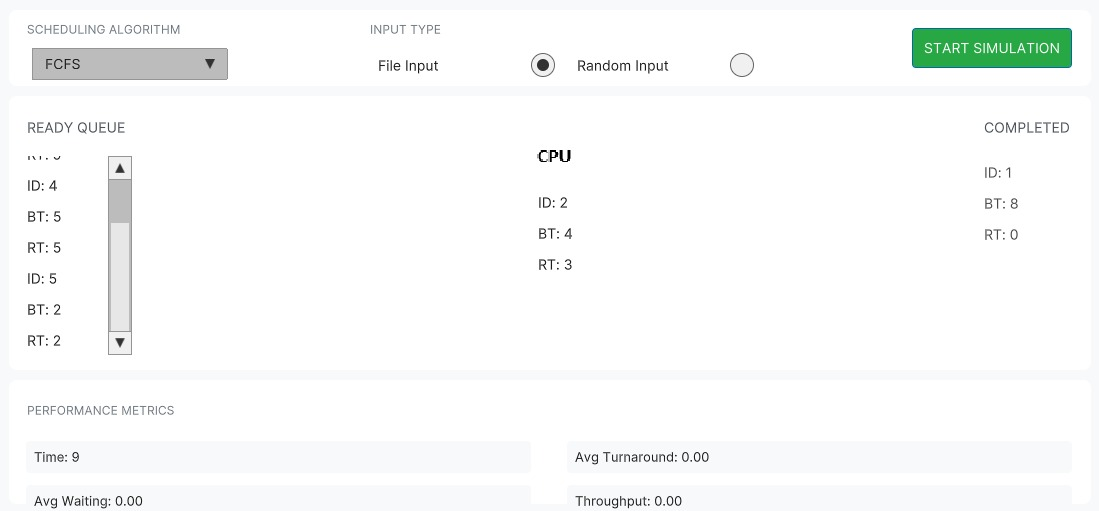
\includegraphics[width=0.8\linewidth]{midSim.jpg}
  \caption{During Simulation State.}
  \label{fig:mid-sim}
\end{figure}

\begin{figure}[H]
  \centering
  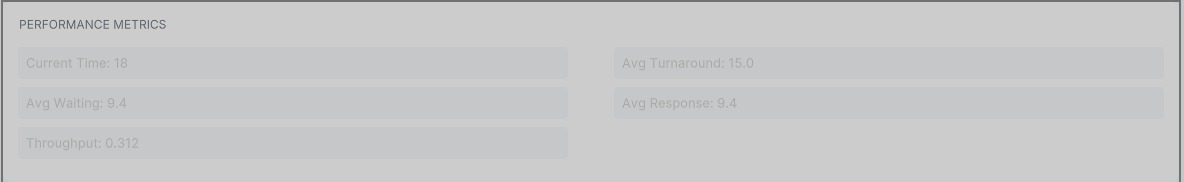
\includegraphics[width=0.8\linewidth]{endSim.jpg}
  \caption{End-of-simulation state (all processes complete).}
  \label{fig:end-sim}
\end{figure}

\subsection{Benchmarking Results}
We record average waiting time, average turnaround time, average response time, and throughput for each algorithm. Table~\ref{tab:results} shows these results.

\begin{table}[H]
  \centering
  \caption{Summary of Results (Quantum = 2)}
  \label{tab:results}
  \begin{tabular}{lrrrr}
      \hline
      Algorithm       & Avg. Waiting & Avg. Turnaround & Avg. Response & Throughput \\
      \hline
      FCFS            & 9.4          & 15.0            & 9.4           & 0.312      \\
      SJF             & 6.2          & 11.8            & 6.2           & 0.424      \\
      Priority        & 7.4          & 13.0            & 7.4           & 0.385      \\
      Round Robin     & 10.6         & 16.2            & 2.4           & 0.308      \\
      Priority+RR     & 7.2          & 12.8            & 3.8           & 0.390      \\
      \hline
    \end{tabular}
\end{table}

\begin{itemize}
  \item \textbf{FCFS} follows strict arrival order: average waiting time = 9.4, average turnaround time = 15.0, average response time = 9.4. Simple to implement, but short tasks arriving later must wait behind long ones, causing the “convoy effect.”
  \item \textbf{SJF} has the lowest average waiting time (6.2) and turnaround time (11.8), but long processes may wait too long.
  \item \textbf{Priority} reduces waiting (7.4) and turnaround (13.0) compared to FCFS, yet low-priority tasks can still be delayed.
  \item \textbf{Round Robin} gives each process a fast start (avg response = 2.4) but raises average waiting (10.6) and turnaround (16.2).
  \item \textbf{Priority + RR} combines both: high-priority jobs start sooner (avg response = 3.8), while waiting (7.2) and turnaround (12.8) stay moderate.
\end{itemize}

\begin{figure}[H]
  \centering
  \resizebox{\columnwidth}{!}{%
  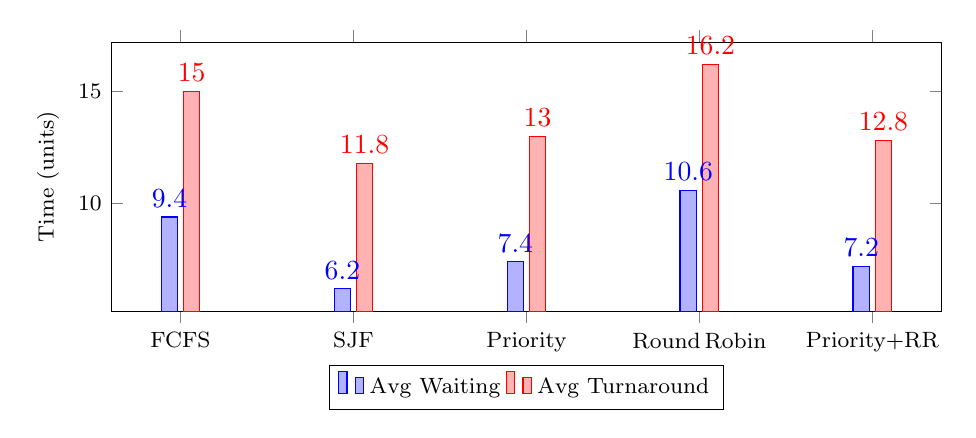
\begin{tikzpicture}
    \begin{axis}[
      ybar,
      bar width=6pt,
      xlabel={Algorithm},
      ylabel={Time (units)},
      symbolic x coords={FCFS,SJF,Priority,Round\,Robin,Priority+RR},
      xtick=data,
      legend style={font=\footnotesize, at={(0.5,-0.2)}, anchor=north, legend columns=2},
      nodes near coords,
      nodes near coords align={vertical},
      tick label style={font=\footnotesize},
      label style={font=\footnotesize},
      width=\linewidth,
      height=5cm,
    ]
      \addplot coordinates {(FCFS,9.4) (SJF,6.2) (Priority,7.4) (Round\,Robin,10.6) (Priority+RR,7.2)};
      \addplot coordinates {(FCFS,15.0) (SJF,11.8) (Priority,13.0) (Round\,Robin,16.2) (Priority+RR,12.8)};
      \legend{Avg Waiting, Avg Turnaround}
    \end{axis}
  \end{tikzpicture}%
  }
  \caption{Comparison of average waiting and turnaround times.}
  \label{fig:perf-plot}
\end{figure}



\end{document}
